\documentclass[11pt]{standalone}
\usepackage{amssymb}
\usepackage{amsmath}
\usepackage[no-math]{fontspec}
\usepackage{unicode-math}
\setmainfont{Libertinus Sans}
\setsansfont{Libertinus Sans}
\setmathfont{Libertinus Math}
\usepackage{pgf,xcolor}
\usepackage{tikz}
\usetikzlibrary{arrows.meta, backgrounds, calc}
\usepackage{pgfplots}
\pgfplotsset{compat=newest}
\usepackage{pifont}

\definecolor{my_darkgray}{HTML}{484949}
\definecolor{my_lightgray}{HTML}{F3F4F4}
\definecolor{my_darkblue}{HTML}{005A94}
\definecolor{my_lightblue}{HTML}{CCDEE9}
\definecolor{my_yellow}{HTML}{FFEC7F}
\definecolor{my_red}{HTML}{E60000}
\definecolor{my_orange}{HTML}{E87846}

\begin{document}
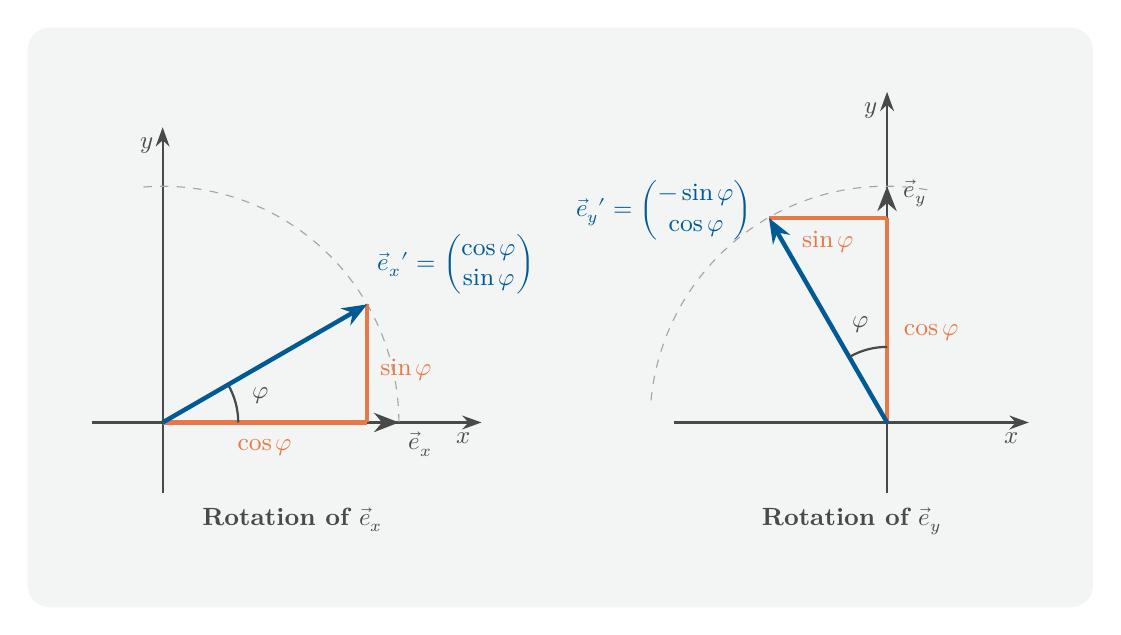
\begin{tikzpicture}[
    show background rectangle,
    background rectangle/.style={fill=my_lightgray, rounded corners=8pt},
    inner frame sep=0.8cm,
    achse/.style={draw=my_darkgray, thick, -{Stealth[length=7pt, width=5pt]}},
    vektor/.style={-{Stealth[length=9pt, width=7pt]}}
]

    % Maßstab: Länge 1 = 3 cm, Drehwinkel phi = 30 Grad
    % cos 30° = 0.866, sin 30° = 0.5

    % ===== Panel 1: Einheitsvektor e_x wird gedreht =====
    \begin{scope}[scale=3]

        \draw[achse] (-0.3,0) -- (1.35,0)
            node[anchor=north east, font=\small, text=my_darkgray] {$x$};
        \draw[achse] (0,-0.3) -- (0,1.25)
            node[anchor=north east, font=\small, text=my_darkgray] {$y$};

        % Einheitskreis als Orientierung
        \draw[draw=my_darkgray!50, thin, dashed] (1,0) arc[start angle=0, end angle=95, radius=1];

        % ursprünglicher Einheitsvektor
        \draw[vektor, draw=my_darkgray, thick] (0,0) -- (1,0);
        \node[font=\small, text=my_darkgray, anchor=north west] at (1.0,0) {$\vec{e}_x$};

        % Komponenten des gedrehten Vektors
        \draw[draw=my_orange, ultra thick] (0,0) -- (0.866,0);
        \draw[draw=my_orange, ultra thick] (0.866,0) -- (0.866,0.5);
        \node[font=\small, text=my_orange, anchor=north] at (0.433,-0.03) {$\cos\varphi$};
        \node[font=\small, text=my_orange, anchor=west] at (0.88,0.22) {$\sin\varphi$};

        % gedrehter Einheitsvektor
        \draw[vektor, draw=my_darkblue, ultra thick] (0,0) -- (0.866,0.5);
        \node[font=\small, text=my_darkblue, anchor=south west] at (0.87,0.5)
            {$\vec{e}_x{}' = \begin{pmatrix} \cos\varphi \\ \sin\varphi \end{pmatrix}$};

        % Drehwinkel
        \draw[draw=my_darkgray, thick] (0.32,0) arc[start angle=0, end angle=30, radius=0.32];
        \node[font=\small, text=my_darkgray] at (15:0.43) {$\varphi$};

        \node[font=\small\bfseries, text=my_darkgray, anchor=north]
            at (0.55,-0.32) {Rotation of $\vec{e}_x$};
    \end{scope}

    % ===== Panel 2: Einheitsvektor e_y wird gedreht =====
    \begin{scope}[xshift=9.2cm, scale=3]

        \draw[achse] (-0.9,0) -- (0.6,0)
            node[anchor=north east, font=\small, text=my_darkgray] {$x$};
        \draw[achse] (0,-0.3) -- (0,1.4)
            node[anchor=north east, font=\small, text=my_darkgray] {$y$};

        % ursprünglicher Einheitsvektor
        \draw[vektor, draw=my_darkgray, thick] (0,0) -- (0,1);
        \node[font=\small, text=my_darkgray, anchor=west] at (0.03,0.97) {$\vec{e}_y$};

        \draw[draw=my_darkgray!50, thin, dashed] (0.17,0.985) arc[start angle=80, end angle=175, radius=1];

        % Komponenten des gedrehten Vektors
        \draw[draw=my_orange, ultra thick] (0,0) -- (0,0.866);
        \draw[draw=my_orange, ultra thick] (0,0.866) -- (-0.5,0.866);
        \node[font=\small, text=my_orange, anchor=west] at (0.03,0.38) {$\cos\varphi$};
        \node[font=\small, text=my_orange, anchor=north] at (-0.25,0.85) {$\sin\varphi$};

        \draw[vektor, draw=my_darkblue, ultra thick] (0,0) -- (-0.5,0.866);
        \node[font=\small, text=my_darkblue, anchor=east] at (-0.53,0.9)
            {$\vec{e}_y{}' = \begin{pmatrix} -\sin\varphi \\ \cos\varphi \end{pmatrix}$};

        \draw[draw=my_darkgray, thick] (0,0.32) arc[start angle=90, end angle=120, radius=0.32];
        \node[font=\small, text=my_darkgray] at (105:0.43) {$\varphi$};

        \node[font=\small\bfseries, text=my_darkgray, anchor=north]
            at (-0.15,-0.32) {Rotation of $\vec{e}_y$};
    \end{scope}

\end{tikzpicture}
\end{document}
